\documentclass{standalone}
\usepackage{tikz}



\begin{document}
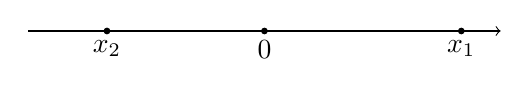
\begin{tikzpicture}
% Draw the real line
  \draw[->] (-3,0) -- (3,0);
  
  % Draw the point 'x' and '0'
  \filldraw (0,0) circle (1pt) node[below] {0};
  \filldraw (2.5,0) circle (1pt) node[below] {$x_1$};
  \filldraw (-2,0) circle (1pt) node[below] {$x_2$};
  
  % Draw the brace and label it
    
  
  
  \end{tikzpicture}
\end{document}